% $HeadURL: https://sbgn.svn.sourceforge.net/svnroot/sbgn/ProcessDiagram/tags/L1V1.3Full/sources/genetic.tex $

\subsection{Glyph: \glyph{Nucleic acid feature}}
\label{sec:genetic}

The \emph{Nucleic acid feature} construct in SBGN is meant to represent a fragment of a macromolecule carrying genetic information.  A common use for this construct is to represent a gene or a transcript.  The label of this EPN and its \emph{units of information} (see \sect{unitInfo}) are often important for making the purpose clear to the reader of a map. A \glyph{nucleic acid feature} is represented by a rectangular container whose bottom half has rounded corners, as shown in \fig{genetic}. This design reminds that we are fundamentally dealing with a unit of information, but this information is carried by a macromolecule.

\begin{figure}[H]
  \centering
  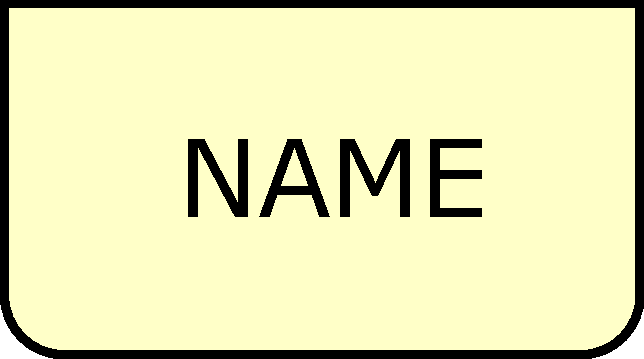
\includegraphics[width = 1.25in]{images/genetic}
  \caption{The \PD glyph for \glyph{nucleic acid feature}.} 
  \label{fig:genetic}
\end{figure}

Examples of \glyph{nucleic acid features} are presented in \fig{NucAcidFeat-examples}.

\begin{figure}[H]
  \centering
  \includegraphics[scale = 0.5]{images/NucAcidFeat-examples}
  \caption{Examples of \glyph{nucleic acid features}. From left to right: gene coding for the 18S ribosomal RNA, gene coding for $\alpha$1-globin, messenger RNA coding for $\alpha$-globin, nuclear factor 1 binding site on the promoter of $\alpha$1-globin gene.}
  \label{fig:NucAcidFeat-examples}
\end{figure}
